\documentclass[a4paper,10pt]{exam}

\usepackage[utf8]{inputenc}
\usepackage[cyr]{aeguill}
\usepackage[francais]{babel}
\usepackage{fullpage}
\usepackage{amsmath}
\usepackage{array}
\usepackage{tikz}
\input kvmacros
\usetikzlibrary{arrows,shapes,trees,patterns,fit,backgrounds,%
decorations.pathreplacing,chains,calc,decorations.pathmorphing,matrix,circuits.logic.CDH}

\ifthenelse{\equal{\detokenize{correction}}{\jobname}}
{\printanswers}
{\noprintanswers}

\title{Architecture des ordinateurs - TD 07}

\author{}
\date{}

\begin{document}
\maketitle

\section{Minterms et Maxterms}
Nous considérerons la fonction logique, $XOR3(A,B,C) = A \oplus B \oplus C$, qui correspond à une porte XOR à trois entrées.
\begin{enumerate}
  \item Donner la table de vérité de $XOR3$.
  \item Écrire les minterms de $XOR3$. 
      \begin{itemize}
        \item Remarquez que la somme des minterms donne une forme disjonctive de $XOR3$.
        \item Remarquez que pour chaque minterm, seule une combinaison unique $(a,b,c)$ rends le terme vrai.
              On identifiera donc le minterm avec la valeur décimale correspondante au mot binaire $abc_2$.
      \end{itemize}
  \item Écrire les minterms de $\overline{XOR3}$. Donner une forme disjonctive de $\overline{XOR3}$.
  \item En utilisant la loi De Morgan, donner une forme conjonctive de $XOR3$. Chaque terme de la forme conjonctive ainsi obtenue est appellé un maxterm. 
  \item Pour chaque maxterm, y a t'il une unique combinaison de $(a,b,c)$ qui rends le maxterm vrai ? 
  \item Pour chaque maxterm, y a t'il une unique combinaison de $(a,b,c)$ qui rends le maxterm faux ? 
  \item Proposez un système permettant d'identifier chaque maxterm avec une valeur décimale. 
\end{enumerate}

\section{Circuits additioneurs (retour)}
\begin{enumerate}
\item Soit deux nombres positifs: $A=a_3a_2a_1a_0$ et $B=b_3b_2b_1b_0$, implémenter
  le circuit de la fonction $C(A,B) = A < B$ \textbf{en utilisant un circuit
    additionneur}.
  \begin{solution}
    On se sert d'un additionneur 5 bits.
    On remarque que $A < B \equiv A - B < 0$.
    On peut obtenir $-B$ en CA2 avec $\overline{B} + 1$.
    Puis on calcule $A-B$ avec l'additionneur 5 bits et on teste le bit de signe
    du résultat.

    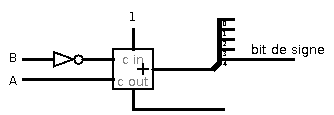
\includegraphics[width=6cm]{comparateur}

  \end{solution}
\end{enumerate}

\section{Quine-McCluskey}
\begin{enumerate}
  \item $f(a,b,c,d) = \Sigma m(4,5,6,7,12,13,14,15)$, on donne la colonne $2^2$
    de la table de QMC. Donner la colonne $2^3$ et retrouver ce résultat par la
    table de Karnaugh.

    \begin{center}
    \begin{tabular}{cll}
              & $2^2$ & $2^3$ \\
      \hline
      4,5,6,7     & \verb!01--!  &\\
      4,5,12,13   & \verb!-10-!  &\\
      4,6,12,14   & \verb!-1-0!  &\\
      \hline
      5,7,13,15   & \verb!-1-1!  &\\
      6,7,14,15   & \verb!-11-!  &\\
      12,13,14,15 & \verb!11--!  &\\
      \hline
    \end{tabular}
    \end{center}

    \begin{solution}
      On retrouve un seul implicant premier: \verb!-1--!.
      L'implicant est donc essentiel et $f=b$
      Sur le tableau de Karnaugh on peut ainsi regrouper tous les 1
      dans un rectangle de taille 8.
    \end{solution}

    \item Donner tous les implicants de la fonction $f(a,b,c) = \Sigma
      m(0,1,5,7)$

      \begin{solution}
        \begin{center}
          \begin{tabular}{cll}
            $2^0$& $2^1$& \\
            \hline
            \verb!0000!& \verb!000-!  &\\
            \hline
            \verb!0001!& \verb!0-01!  &\\
            \hline
            \verb!0101!& \verb!01-1!  &\\
            \hline
            \verb!0111!&  &\\
            \hline
          \end{tabular}
        \end{center}

        On trouve trois implicants. Les implicants 1 et 3 sont essentiels.
        \begin{tabular}{ccccc}
          &0&1&5&7\\
          \hline
       0,1&X&X& & \\
       1,5& &X&X& \\
       5,7& & &X&X\\
        \end{tabular}
      \end{solution}


    \item On considère la table des implicants ci-dessous.
      \begin{enumerate}
        \item Simplifiez la et déduisez en une forme disjonctive minimale.
          \begin{solution}
            On peut remarquer pour la simplification que $\overline{c}d$ est
            inclus dans $bd$.
          \end{solution}
        \item Donnez toutes les formes disjonctives minimales possibles.
          \begin{solution}
            \begin{itemize}
              \item $bd + \overline{a}b$
              \item $bd + b\overline{c}$
              \item $\overline{a}b + b\overline{c}$
              \item $\overline{a}b + \overline{c}d$
            \end{itemize}
          \end{solution}
      \end{enumerate}

      \begin{center}
      \begin{tabular}{c|c|c|c|c|}
        & $4$& $5$ & $7$ & $13$\\
                       \hline
        $b.d$           &   & X & X & X \\
        $b.\overline{c}$& X & X &   & X \\
        $\overline{a}.b$& X & X & X &   \\
        $\overline{c}.d$&   & X &   & X
      \end{tabular}
      \end{center}
    \item Mêmes questions pour la table des implicants ci-dessous.
      \begin{center}
      \begin{tabular}{c|c|c|c|c|c|c|c|c|c|c|}
                                   &0&1&2&5&6&7&8&9&10&14\\
                                   \hline
        $\overline{b}.\overline{c}$ &X&X& & & & &X&X&  &  \\
        $\overline{b}.\overline{d}$ &X& &X& & & &X& &X &  \\
        $c.\overline{d}$            & & &X& &X& & & &X &X \\
        $\overline{a}.\overline{c}.d$& &X& &X& & & & &  &  \\
        $\overline{a}.b.d$           & & & &X& &X& & &  &  \\
        $\overline{a}.b.c$           & & & & &X&X& & &  &
      \end{tabular}
      \end{center}

      \begin{solution}
        $\overline{b}.\overline{c} + \overline{c}.d + \overline{a}.b.d$
      \end{solution}

    \item $f(a,b,c,d)=\Sigma m(4,8,10,11,12,15) + d(9,14)$:
      \begin{enumerate}
        \item Déterminer les nombres binaires correspondant aux décimaux et les
          répartir en groupes (en fonction du nombre de bits à 1).
        \item Déterminer les implicants premiers de la fonction.
        \item Construire la table des implicants et déterminer les implicants
          premiers essentiels.
        \item Déterminer une solution minimale.
        \item Déterminer toutes les solutions minimales.
      \end{enumerate}

      \begin{solution}
        (La table ci-dessous a été générée avec l'excellent logiciel libre
        Bmin de J. Zelenka)

        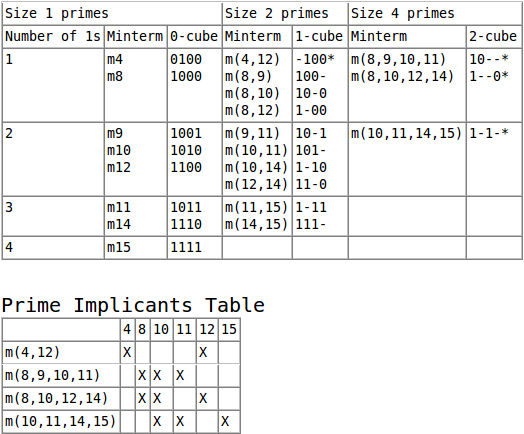
\includegraphics[width=8cm]{QMC1}

        Le premier et dernier implicants sont essentiels. On aboutit à deux
        expressions minimales possibles:
        \begin{itemize}
          \item $b.\overline{c}.\overline{d} + a\overline{d} + a.c$
          \item $b.\overline{c}.d + a\overline{b} + a.c$
        \end{itemize}
      \end{solution}

    \item Simplifier avec la méthode de QMC l'expression $f(a,b,c,d,e)=\Sigma
      m(0,2,3,5,7,9,11,13,14,16,18,24,26,28,30)$.
      \begin{solution}

        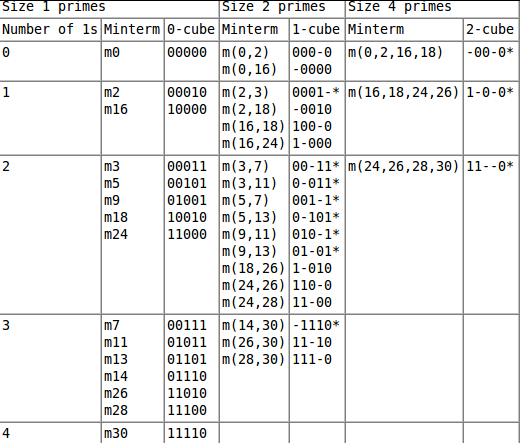
\includegraphics[width=8cm]{QMC2a}

        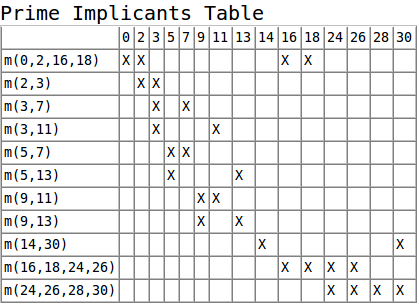
\includegraphics[width=6cm]{QMC2b}


        Une solution minimale est: $\overline{E}.\overline{C}.\overline{B} +
        \overline{E}.D.C.B + \overline{E}.B.A + E.D.\overline{B}.\overline{A} +
        E.\overline{D}.\overline{C}.\overline{A} + E.\overline{C}.B.\overline{A}$.
      \end{solution}
\end{enumerate}

\section{Circuit Multiplieur}

On souhaite réaliser un circuit multiplieur.
\begin{enumerate}
  \item Réaliser à la main la multiplication de $1011 \times 1100$.
  \item Construire un circuit qui multiplie deux nombres positifs
    sur 4 bits. Vous disposez d'additioneurs 4 bits.
    \begin{solution}
      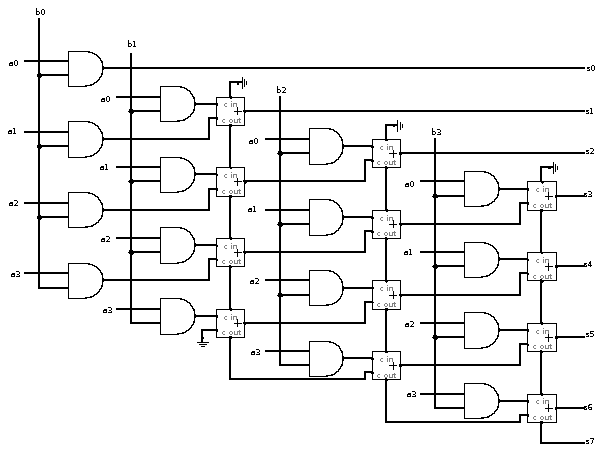
\includegraphics[width=10cm]{4-mult}
    \end{solution}

  \item Ce schéma marche t'il pour des entrées codées en complément à 2.
    Si ce n'est pas le cas, comment faudrait-il le modifier ?
    \begin{solution}
      On veut multiplier A et B, mais cette fois ci ils peuvent être signés.
      On décompose le produit de la manière suivante :
      $$B \times A = ( -b_3 \times 2^3 + b_2 \times 2^2 + b_1 \times 2^1 + b_0 \times 2^0) \times A$$
      Ici c'est la définition de B en CA2 où le dernier bit est bit de signe. Puis par distributivité du produit :
      $$B \times A = (A \times( -b_3)) \times 2^3 + (A \times b_2) \times 2^2 + ... + (A \times b_0)$$

      Maintenant il suffit d'additionner les facteurs (ou produits partiels) entre eux.
      \\Deux remarques importantes:
      \begin{itemize}
        \item Le terme $(A \times (-b_3)) \times 2^3$ peut être réécrit $(-A \times b_3) \times 2^3$.
	  Or par définition du CA2, $-A = \overline{A} + 1$	, c'est pourquoi on complémente 
	  A lorsque b3 est à 1.
	\item Lorsque l'on additionne des produits partiels en CA2, il faut faire 
	  attention à propager le bit de signe. Par exemple, supposons que le résultat 
	  du premier étage est 11 (-1 sur deux bits) et le résultat du deuxième étage 
	  est 100 (-4 sur trois bits). Si on additionne sans extension de signe 
	  $11 + 100 = 111$, le résultat est -1 sur 3 bits ce qui est faux.
	  C'est pourquoi il faut étendre le bit de signe $111 + 100 = 1011$ : le
	  résultat devient $-8 + 2 + 1 = -5$, ce qui est correct.
      \end{itemize}

      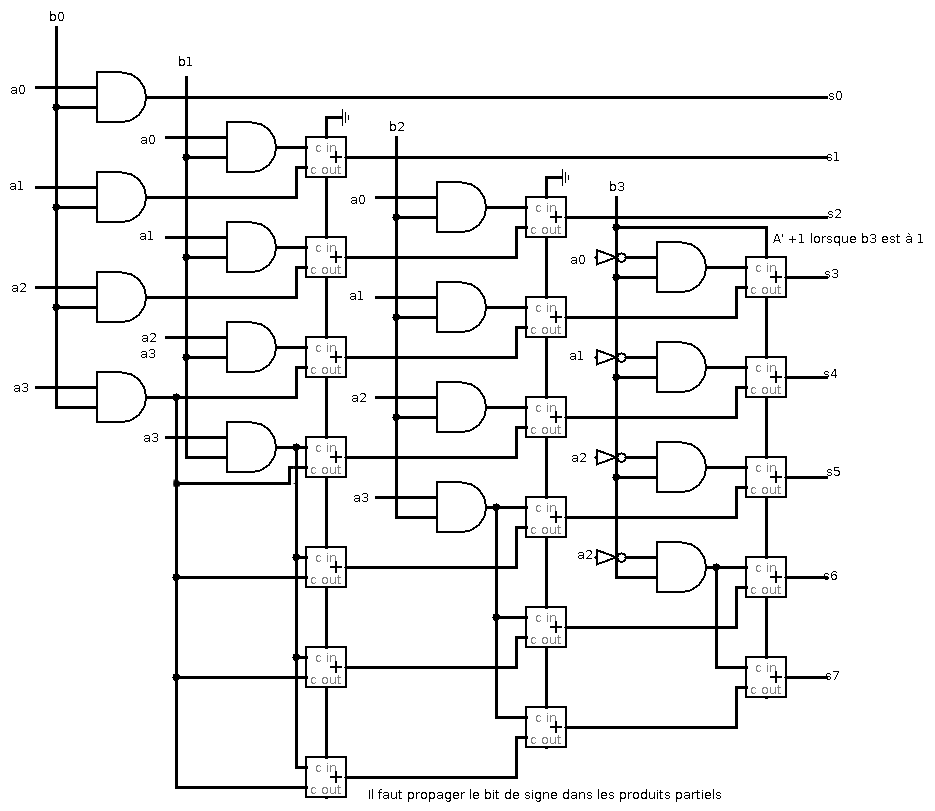
\includegraphics[width=10cm]{4-mult-CA-2}
      
    \end{solution}

\end{enumerate}

\end{document}
